\documentclass[12pt,twoside]{article}


\newcommand{\reporttitle}{Blockchain-based solutions and their feasibility in the financial world}
\newcommand{\reportauthor}{Michael Carneciu}
\newcommand{\reporttype}{BEng Individual Project}
\newcommand{\cid}{09...}

% include files that load packages and define macros
%%%%%%%%%%%%%%%%%%%%%%%%%%%%%%%%%%%%%%%%%
% University Assignment Title Page 
% LaTeX Template
% Version 1.0 (27/12/12)
%
% This template has been downloaded from:
% http://www.LaTeXTemplates.com
%
% Original author:
% WikiBooks (http://en.wikibooks.org/wiki/LaTeX/Title_Creation)
%
% License:
% CC BY-NC-SA 3.0 (http://creativecommons.org/licenses/by-nc-sa/3.0/)
% 
% Instructions for using this template:
% This title page is capable of being compiled as is. This is not useful for 
% including it in another document. To do this, you have two options: 
%
% 1) Copy/paste everything between \begin{document} and \end{document} 
% starting at \begin{titlepage} and paste this into another LaTeX file where you 
% want your title page.
% OR
% 2) Remove everything outside the \begin{titlepage} and \end{titlepage} and 
% move this file to the same directory as the LaTeX file you wish to add it to. 
% Then add \input{./title_page_1.tex} to your LaTeX file where you want your
% title page.
%
%----------------------------------------------------------------------------------------
%	PACKAGES AND OTHER DOCUMENT CONFIGURATIONS
%----------------------------------------------------------------------------------------
\usepackage[table,xcdraw]{xcolor}
\usepackage{ifxetex}
\usepackage{textpos}
\usepackage[numbers]{natbib}
\usepackage{kpfonts}
\usepackage[a4paper,hmargin=2.8cm,vmargin=2.0cm,includeheadfoot]{geometry}
\usepackage{ifxetex}
\usepackage{stackengine}
\usepackage{tabularx,longtable,multirow,caption}%hangcaption
\usepackage{fncylab} %formatting of labels
\usepackage{fancyhdr}
\usepackage{color}
\usepackage[tight,ugly]{units}
\usepackage{float}
\usepackage[english]{babel}
\usepackage{amsmath}
\usepackage{graphicx}
\usepackage[colorinlistoftodos]{todonotes}
\usepackage{dsfont}
\usepackage{epstopdf} % automatically replace .eps with .pdf in graphics
\usepackage{natbib}
\usepackage{array}
\usepackage{latexsym}
\usepackage{etoolbox}
\usepackage[hyphenbreaks]{breakurl}
\usepackage[hyphens]{url}
\usepackage{enumerate} % for numbering with [a)] format 
\usepackage{subcaption}
\usepackage{smartdiagram}
\usepackage{booktabs}

%\documentclass[xcolor=table]{beamer}

\ifxetex
\usepackage{fontspec}
\setmainfont[Scale=.8]{OpenDyslexic-Regular}
\else
\usepackage[pdftex,hypertexnames=false,colorlinks]{hyperref} % provide links in pdf
\hypersetup{pdftitle={},
  pdfsubject={}, 
  pdfauthor={\reportauthor},
  pdfkeywords={}, 
  pdfstartview=FitH,
  pdfpagemode={UseOutlines},% None, FullScreen, UseOutlines
  bookmarksnumbered=true, bookmarksopen=true, colorlinks,
    citecolor=black,%
    filecolor=black,%
    linkcolor=black,%
    urlcolor=black}
\usepackage[all]{hypcap}
\fi

\usepackage{tcolorbox}

% various theorems
\usepackage{ntheorem}
\theoremstyle{break}
\newtheorem{lemma}{Lemma}
\newtheorem{theorem}{Theorem}
\newtheorem{remark}{Remark}
\newtheorem{definition}{Definition}
\newtheorem{proof}{Proof}

% example-environment
\newenvironment{example}[1][]
{ 
\vspace{4mm}
\noindent\makebox[\linewidth]{\rule{\hsize}{1.5pt}}
\textbf{Example #1}\\
}
{ 
\noindent\newline\makebox[\linewidth]{\rule{\hsize}{1.0pt}}
}



%\renewcommand{\rmdefault}{pplx} % Palatino
% \renewcommand{\rmdefault}{put} % Utopia

\ifxetex
\else
\renewcommand*{\rmdefault}{bch} % Charter
\renewcommand*{\ttdefault}{cmtt} % Computer Modern Typewriter
%\renewcommand*{\rmdefault}{phv} % Helvetica
%\renewcommand*{\rmdefault}{iwona} % Avant Garde
\fi

\setlength{\parindent}{0em}  % indentation of paragraph

\setlength{\headheight}{14.5pt}
\pagestyle{fancy}
\fancyfoot[ER,OL]{\thepage}%Page no. in the left on
                                %odd pages and on right on even pages
\fancyfoot[OC,EC]{\sffamily }
\renewcommand{\headrulewidth}{0.1pt}
\renewcommand{\footrulewidth}{0.1pt}
\captionsetup{margin=10pt,font=small,labelfont=bf}


%--- chapter heading

\def\@makechapterhead#1{%
  \vspace*{10\p@}%
  {\parindent \z@ \raggedright %\sffamily
        %{\Large \MakeUppercase{\@chapapp} \space \thechapter}
        %\\
        %\hrulefill
        %\par\nobreak
        %\vskip 10\p@
    \interlinepenalty\@M
    \Huge \bfseries 
    \thechapter \space\space #1\par\nobreak
    \vskip 30\p@
  }}

%---chapter heading for \chapter*  
\def\@makeschapterhead#1{%
  \vspace*{10\p@}%
  {\parindent \z@ \raggedright
    \sffamily
    \interlinepenalty\@M
    \Huge \bfseries  
    #1\par\nobreak
    \vskip 30\p@
  }}
  



% %%%%%%%%%%%%% boxit
\def\Beginboxit
   {\par
    \vbox\bgroup
	   \hrule
	   \hbox\bgroup
		  \vrule \kern1.2pt %
		  \vbox\bgroup\kern1.2pt
   }

\def\Endboxit{%
			      \kern1.2pt
		       \egroup
		  \kern1.2pt\vrule
		\egroup
	   \hrule
	 \egroup
   }	

\newenvironment{boxit}{\Beginboxit}{\Endboxit}
\newenvironment{boxit*}{\Beginboxit\hbox to\hsize{}}{\Endboxit}



\allowdisplaybreaks

\makeatletter
\newcounter{elimination@steps}
\newcolumntype{R}[1]{>{\raggedleft\arraybackslash$}p{#1}<{$}}
\def\elimination@num@rights{}
\def\elimination@num@variables{}
\def\elimination@col@width{}
\newenvironment{elimination}[4][0]
{
    \setcounter{elimination@steps}{0}
    \def\elimination@num@rights{#1}
    \def\elimination@num@variables{#2}
    \def\elimination@col@width{#3}
    \renewcommand{\arraystretch}{#4}
    \start@align\@ne\st@rredtrue\m@ne
}
{
    \endalign
    \ignorespacesafterend
}
\newcommand{\eliminationstep}[2]
{
    \ifnum\value{elimination@steps}>0\leadsto\quad\fi
    \left[
        \ifnum\elimination@num@rights>0
            \begin{array}
            {@{}*{\elimination@num@variables}{R{\elimination@col@width}}
            |@{}*{\elimination@num@rights}{R{\elimination@col@width}}}
        \else
            \begin{array}
            {@{}*{\elimination@num@variables}{R{\elimination@col@width}}}
        \fi
            #1
        \end{array}
    \right]
    & 
    \begin{array}{l}
        #2
    \end{array}
    &%                                    moved second & here
    \addtocounter{elimination@steps}{1}
}
\makeatother

%% Fast macro for column vectors
\makeatletter  
\def\colvec#1{\expandafter\colvec@i#1,,,,,,,,,\@nil}
\def\colvec@i#1,#2,#3,#4,#5,#6,#7,#8,#9\@nil{% 
  \ifx$#2$ \begin{bmatrix}#1\end{bmatrix} \else
    \ifx$#3$ \begin{bmatrix}#1\\#2\end{bmatrix} \else
      \ifx$#4$ \begin{bmatrix}#1\\#2\\#3\end{bmatrix}\else
        \ifx$#5$ \begin{bmatrix}#1\\#2\\#3\\#4\end{bmatrix}\else
          \ifx$#6$ \begin{bmatrix}#1\\#2\\#3\\#4\\#5\end{bmatrix}\else
            \ifx$#7$ \begin{bmatrix}#1\\#2\\#3\\#4\\#5\\#6\end{bmatrix}\else
              \ifx$#8$ \begin{bmatrix}#1\\#2\\#3\\#4\\#5\\#6\\#7\end{bmatrix}\else
                 \PackageError{Column Vector}{The vector you tried to write is too big, use bmatrix instead}{Try using the bmatrix environment}
              \fi
            \fi
          \fi
        \fi
      \fi
    \fi
  \fi 
}  
\makeatother

\robustify{\colvec}

%%% Local Variables: 
%%% mode: latex
%%% TeX-master: "notes"
%%% End: 
 % various packages needed for maths etc.
% quick way of adding a figure
\newcommand{\fig}[3]{
 \begin{center}
 \scalebox{#3}{\includegraphics[#2]{#1}}
 \end{center}
}

%\newcommand*{\point}[1]{\vec{\mkern0mu#1}}
\newcommand{\ci}[0]{\perp\!\!\!\!\!\perp} % conditional independence
\newcommand{\point}[1]{{#1}} % points 
\renewcommand{\vec}[1]{{\boldsymbol{{#1}}}} % vector
\newcommand{\mat}[1]{{\boldsymbol{{#1}}}} % matrix
\newcommand{\R}[0]{\mathds{R}} % real numbers
\newcommand{\Z}[0]{\mathds{Z}} % integers
\newcommand{\N}[0]{\mathds{N}} % natural numbers
\newcommand{\nat}[0]{\mathds{N}} % natural numbers
\newcommand{\Q}[0]{\mathds{Q}} % rational numbers
\ifxetex
\newcommand{\C}[0]{\mathds{C}} % complex numbers
\else
\newcommand{\C}[0]{\mathds{C}} % complex numbers
\fi
\newcommand{\tr}[0]{\text{tr}} % trace
\renewcommand{\d}[0]{\mathrm{d}} % total derivative
\newcommand{\inv}{^{-1}} % inverse
\newcommand{\id}{\mathrm{id}} % identity mapping
\renewcommand{\dim}{\mathrm{dim}} % dimension
\newcommand{\rank}[0]{\mathrm{rk}} % rank
\newcommand{\determ}[1]{\mathrm{det}(#1)} % determinant
\newcommand{\scp}[2]{\langle #1 , #2 \rangle}
\newcommand{\kernel}[0]{\mathrm{ker}} % kernel/nullspace
\newcommand{\img}[0]{\mathrm{Im}} % image
\newcommand{\idx}[1]{{(#1)}}
\DeclareMathOperator*{\diag}{diag}
\newcommand{\E}{\mathds{E}} % expectation
\newcommand{\var}{\mathds{V}} % variance
\newcommand{\gauss}[2]{\mathcal{N}\big(#1,\,#2\big)} % gaussian distribution N(.,.)
\newcommand{\gaussx}[3]{\mathcal{N}\big(#1\,|\,#2,\,#3\big)} % gaussian distribution N(.|.,.)
\newcommand{\gaussBig}[2]{\mathcal{N}\left(#1,\,#2\right)} % see above, but with brackets that adjust to the height of the arguments
\newcommand{\gaussxBig}[3]{\mathcal{N}\left(#1\,|\,#2,\,#3\right)} % see above, but with brackets that adjust to the height of the arguments
\DeclareMathOperator{\cov}{Cov} % covariance (matrix) 
\ifxetex
\renewcommand{\T}[0]{^\top} % transpose
\else
\newcommand{\T}[0]{^\top}
\fi
% matrix determinant
\newcommand{\matdet}[1]{
\left|
\begin{matrix}
#1
\end{matrix}
\right|
}



%%% various color definitions
\definecolor{darkgreen}{rgb}{0,0.6,0}

\newcommand{\blue}[1]{{\color{blue}#1}}
\newcommand{\red}[1]{{\color{red}#1}}
\newcommand{\green}[1]{{\color{darkgreen}#1}}
\newcommand{\orange}[1]{{\color{orange}#1}}
\newcommand{\magenta}[1]{{\color{magenta}#1}}
\newcommand{\cyan}[1]{{\color{cyan}#1}}


% redefine emph
\renewcommand{\emph}[1]{\blue{\bf{#1}}}

% place a colored box around a character
\gdef\colchar#1#2{%
  \tikz[baseline]{%
  \node[anchor=base,inner sep=2pt,outer sep=0pt,fill = #2!20] {#1};
    }%
}%
 % short-hand notation and macros
\usepackage{verbatim}
\bibstyle{natbib}

\graphicspath{{/Users/mikecar/Desktop/Blockchain-dizzy/imgs/}}
%%%%%%%%%%%%%%%%%%%%%%%%%%%%

\begin{document}
% front page
% Last modification: 2016-09-29 (Marc Deisenroth)
\begin{titlepage}

\newcommand{\HRule}{\rule{\linewidth}{0.5mm}} % Defines a new command for the horizontal lines, change thickness here


%----------------------------------------------------------------------------------------
%	LOGO SECTION
%----------------------------------------------------------------------------------------

\begin{center} % Center remainder of the page

\includegraphics[width = 11cm]{./figures/imperial}\\[0.5cm] 
\vspace{2.5cm}

%----------------------------------------------------------------------------------------
%	HEADING SECTIONS
%----------------------------------------------------------------------------------------
\textsc{\LARGE \reporttype}\\[1.5cm] 
\textsc{\Large Imperial College London}\\[0.5cm] 
\textsc{\large Department of Computing}\\[0.5cm] 
%----------------------------------------------------------------------------------------
%	TITLE SECTION
%----------------------------------------------------------------------------------------

\HRule \\[0.4cm]
{ \huge \bfseries \reporttitle}\\ % Title of your document
%{ \large \bfseries \reportsubtitle}\\
\HRule \\[1.5cm]
\end{center}
%----------------------------------------------------------------------------------------
%	AUTHOR SECTION
%----------------------------------------------------------------------------------------

%\begin{minipage}{0.4\hsize}

\vspace{1cm}
\begin{minipage}{0.4\hsize}
\flushleft
\textsc{Author:}

Michael Carneciu\\
\end{minipage}
\hfill
\begin{minipage}{0.4\hsize}
\flushright
\textsc{Supervisor:}

Dr Anandha Gopalan\\
\vspace{0.5cm}
\textsc{Second Marker:}

Dr Naranker Dulay
\end{minipage}

\vspace{4cm}
\makeatletter
\begin{center}
\@date 
\end{center}

\vfill % Fill the rest of the page with whitespace



\makeatother


\end{titlepage}



\tableofcontents
\newpage
%%%%%%%%%%%%%%%%%%%%%%%%%%%% Main document
%\section{Abstract}
%\section{Acknowledgements}
%I would like to thank Dr Anandha Gopalan for his help and support throughout the project. bla bla. I would like to thank my friends Dom, Ab and Elias for supporting me throughout and showing me that a final year student can still have fun, Giacomo for helping me overcome my crises and David for always picking up my mood. Special thanks go to my mother and the rest of my family for supporting me during my Imperial years.
\section{Introduction}
\label{sec:Introduction}
\subsection{Motivation}
\label{sub:Motivation}
Time has gradually become one of the most important currencies to humankind. Fortunately, we now benefit from instant messaging, instant information sharing and high speed connections between people. However, the financial world is stuck in the past - there have not been any revolutionary computational developments able to refresh the industry and bring it to the standard of the current world. One of the reasons for this could be the rigidity of the industry with regards to change. Migrations are dangerous considering the fact that banks deal with large sums of money and any computational issue could have devastating effects to their operation (record loss or incorrect migration protocols leading to the loss of capital) \cite{bankrisk}.
\\ \\
This deprecated infrastructure leads to processing times of up to T+3 \cite{TTimes} (meaning that it takes 3 days from the moment when a transaction has been initialised to the moment when the funds and assets have changed ownership on the ledger). The traditional way of performing transactions is also error-prone because of the inevitable human interaction \cite{humanrisk}. Any mistake made when a trade is being performed adds even more latency to the transaction time. Since time is so valuable to us nowadays, there is a clear need to update the way banks do business. However, to be able to adopt any new methods and technologies, these would have to be thoroughly analysed to verify they can be held to the standards required by the financial world.
\\ \\ 
This is a particularly interesting topic because it shows the way Computing seeps into all areas of life. Not only does it constitute the basis for any process, through hardware and low-level software, but it is also able to help industries achieve their full potential. The financial industry has been one of the drivers of Computing in the past, with their usage of databases to manage records pushing development in this area. Now, it is time once again for banks to lead the way by implementing and adopting computational solutions to deal with the issues presented.
\subsection{Objectives}
\label{sub:Objectives}
Imagine Alice and Bob want to perform a simplified version of a transaction. Alice has \pounds 200 in her digital wallet and Bob has 10 shares of stock A (each priced at \pounds 10). The two of them want to execute the trade, Alice buying 10 shares from Bob worth \pounds 100. Now, this transaction would immediately get executed if Alice had enough funds in her wallet, Bob had enough shares and the trade details were correctly matched by our system. 
\\ \\
The record of the trade is now available on the ledger for them to see it, without the transaction having to go through a Clearing House (an intermediary between buyers and sellers of financial instruments). This is graphically depicted in \ref{fig:scheme}. 
\begin{figure}[H]
\centering
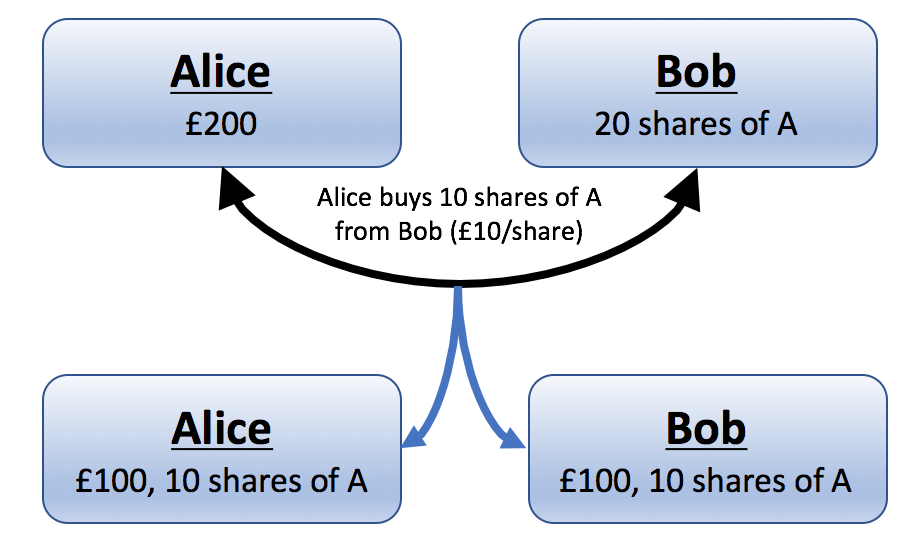
\includegraphics[width=0.7\textwidth]{alicebob.png}
\caption{Simplified schematic representation of a trade}
\centering
\label{fig:scheme}
\end{figure}

In this ideal system, there are no mistakes that can be done (if the details do not match, the trade is not executed), so the transaction is irreversible now. And since Alice's wallet now contains \pounds 100 and 10 shares of stock A, we add the benefit of multi-asset digital wallets. Therefore, with this ideal system, the clearing and settlement part of a transaction would no longer last for days and cost banks huge amounts of money.
\\ \\
But, as mentioned before, any solution to the problems the financial industry faces has to be thoroughly researched before it can get the level of confidence necessary. Trust is crucial when dealing with money and losing it is not an option. To tackle latency in performing trades and eliminating as much human interaction as possible from this process we can think of a blockchain based solution, potentially related to a cryptocurrency-based system. A blockchain is defined as a distributed, decentralised transaction ledger which records publicly all transactions made by the contributing parties \cite{pwc}. This started with the creation of Bitcoin by Satoshi Nakamoto and has increasingly become a popular alternative to common financial practices. But can this be fully adopted in the financial world to replace traditional banking?
\\ \\
This paper will explore proposed solutions, including general blockchains (such as Bitcoin's BC or BigchainDB), financial blockchains (Ripple and BitShares) and blockchain-inspired financial solutions (Corda). We need to establish a set of requirements and investigate the applicability of each system by looking at their salient features and how they compare against the required features. It should be clear that we are not expecting any of these to be completely appropriate and that we are rather investigating which system is the closest to the ideal solution and what features can be sacrificed. It is a given that most of the features needed in this new system will be driven by the current features of traditional banking solutions. However, it must be noted that some of these have to be adapted to satisfy the new infrastructure and frameworks used.
\\ \\
After choosing the most appropriate system to extend, a series of supporting applications will be implemented. These look at different salient features and how they differ from the current processes or from other solutions. They will also attempt to test any claims made without formal proofs. Moreover, there will be a theoretical analysis for some of the requirements, supported by statistical data and proofs. Another goal of the project is to develop a demonstrative application that wraps all the useful behaviour researched in the paper into a product that can be used by people without programming background. The aim of this is to show that the Internet of Finance \cite{CMM:RN} is an achievable concept. Finally, the paper will look at some social implications such an implementation would have, particularly the challenges such a system faces from a reputational and legal standpoint.

\newpage
\section{Background}
\label{sec:Background}
Traditional banking has lost its appeal in this digital era. Fast payments, done via your mobile phone are the norm now. The push from the industry to focus the attention on the individual has been able to transform the customer side of the business. That being said, the infrastructure for corporate banking follows the same monolithic pattern as 40 years ago and digital developments have been slow throughout \cite{slow}. Although there have been attempts to modify this and modularise everything, perhaps the best solution is to start with a clean slate. Why is this so important now? As mentioned before, latencies and human errors are the main drivers of this move to update the systems. But perhaps we should also be looking at the cost of the current applications as opposed to a simpler, modern protocol. Industry experts estimate that \$15bn-\$20bn could be saved in costs by adopting a distributed ledger technology by 2022. These costs mainly come from the fees for cross-border payments, securities trading and regulatory compliance \cite{Clearing:cost}.
\\ \\
However, a ``deadline" of 5 years for implementing a completely new base-layer system might seem daunting. Let's now look at the features of traditional banking which will help us gather the requirements for the new distributed ledger technology. 
\subsection{Traditional Banking}
\label{sub:TraditionalBanking}
The banking ecosystem is very complex. This paper will give a brief description of the areas touched and discussed in it: financial instruments, the life cycle of a trade (for securities) and important institutions like Clearing Houses (and their roles). 

\subsubsection{Financial Instruments}
\label{sub:FinancialInstruments}
Financial instruments are assets that can be traded \cite{FA}. The assets can be multiple things: cash, ownership or a contract that gives the right to deliver or receive another financial instrument. For example, securities are financial instruments and their issuer is the company that issues it. They can be stocks (ownership positions in a publicly traded company), bonds (debt investments at a certain interest rate) or options (the right, but not obligation to ownership) \cite{Security}. In contrast with the options, futures are financial contracts that obligate the buyer to purchase an asset at a later date. All of them are traded differently and have different standards. 
\\ \\
There are 2 important dates for any securities trade: the transaction time and the settlement time. The former is related to the moment when the transaction occurs, while the latter represents the day in which ownership is transferred. This is further discussed in section \ref{sub:LCOAT}. However, to give an example of a downside of the current banking system, securities have various settlement periods. Currently, it takes 3 days for a stock trade to be settled. That means that if a person buys a stock on Monday, that transaction will be settled on Thursday \cite{TTimes}. This is important to know because it determines when exactly the client owns the stock or receives the money.
\subsubsection{Life Cycle of a Trade}
\label{sub:LCOAT}
This section aims to present a high-level view of the steps a trade goes through, from the decision to initiate a trade to the final settlement part. For the examples given, we will be focusing on an order to buy some shares in the stock market. The five main parts of a trade are as follows \cite{TradeCycle}:

\begin{figure}[H]
\centering
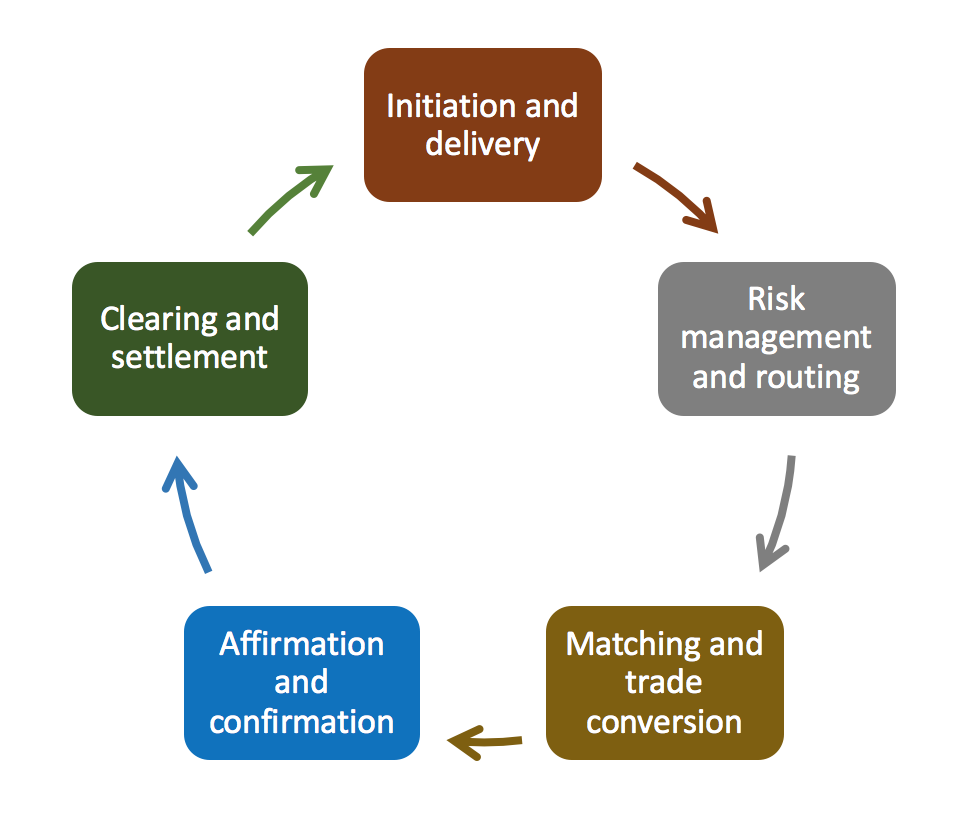
\includegraphics[width=0.9\textwidth]{lcoat.png}
\centering
\label{fig:scheme}
\end{figure}

In the \textbf{initiation and delivery} stage, the client places the order to the broker. This can be done via any existent communication channel (phone, fax, online trading). It is now the broker's responsibility to register all the details of the order correctly and accurately so that no errors appear during the processing stage. Next up, in the \textbf{risk management and routing} step, the broker has to perform critical checks to ensure the client is a reliable source. Moreover, to control the risk, the broker also has to check whether the client has enough margin money (i.e. a sufficient balance to perform the trade - calculated based on the level of exposure and risk that the broker would be facing) or enough stocks (depending on the order type - buy or sell) to place the order. After the suite of checks finishes successfully, the broker gets a confirmation about the order and its execution begins or is delayed according to the terms defined by the two parties. 
\\ \\
The \textbf{matching and conversion} part follows. All such orders are collated and sent to the exchange, which allots the best price available to investors. Once the order is executed, it is converted into a trade and the broker receives a confirmation message that he has to pass over to the client. For the fourth step, \textbf{affirmation and confirmation}, there is a custodian agency that assists insistutions in the clearing and settlement activities. They receive all information existent about trades and review their terms. If differences are found between the desired order and the actual trade (security mismatch, incorrect order type, different charges than the ones agreed upon), the custodian rejects it; otherwise, the broker receives confirmation. 
\\ \\
The last step encompassed a plethora of operations, which is why the delay introduced by Clearing Houses is often very high. \textbf{Clearing} refers to the net obligation at the end of a trading period (say, a day). To better understand this, we can take the following example. Alice buys 100 shares in Company A, for \pounds 100. She then sells 10 shares in Company A (for \pounds 10) and then she sells 10 more. Overall, in the clearing stage, she has 80 shares in Company A and spent \pounds 80 (\pounds 100 initially, then received \pounds 10 twice from the shares sold). Now, in the \textbf{settlement} part of the trade, the shares and money have to transfer ownership. Therefore, what esentially happens is that \pounds 80 go out of Alice's account and 80 shares are credited to her account. At this point, the trade is considered complete \cite{TradeCycle2}.

\subsubsection{Risks and Bottlenecks}
\label{sub:Risks}
It is clear that the main bottleneck appears in the last step of the trade's life cycle. Usually the wait to have your account credited goes over 2 days. Not only is this an inconvenience for customers, but it is also an element of high risk. The Clearing Houses, which deal with the entire clearing and settlement process are subjected to default risk from any of the clearing members. If a clearing member defaults, the Clearing House is still under obligation to fulfill its duty for the other party in the trade. These costs are varied and depends on the type of financial instrument trades (futures or options) \cite{CHRisk}. Operational risk can also occur through system failure, human errors or inadequate management. Obviously, the usage of another entity in the trading cycle has many implications - most of them negative, from a productivity point of view.
\\ \\
Since latency and risk are heightened by the presence of Clearing Houses, their role should either be completely replaced or their responsabilities shrunk in such a way to take on less responsibility. This sounds like an ideal situation that is hard to reach by using the current infrastructure. There is not a way to record transactions in a short period of time, avoiding the detour via the Clearing House. However, the possible replacement of the deprecated infrastructure discussed above could facilitate development and getting to ``immediate" clearing and settlement of trades. (To be noted that ``immediate" will become one of the requirements for the system that will be presented in this paper. However, this term is relative to the current process and can last as long as 15 minutes. An upper bound will be put on this, depending on further research done in subsequent sections.) \\ \\
\begin{figure}[!htb]
    \centering
    \begin{subfigure}[b]{0.48\textwidth}
    	\centering
        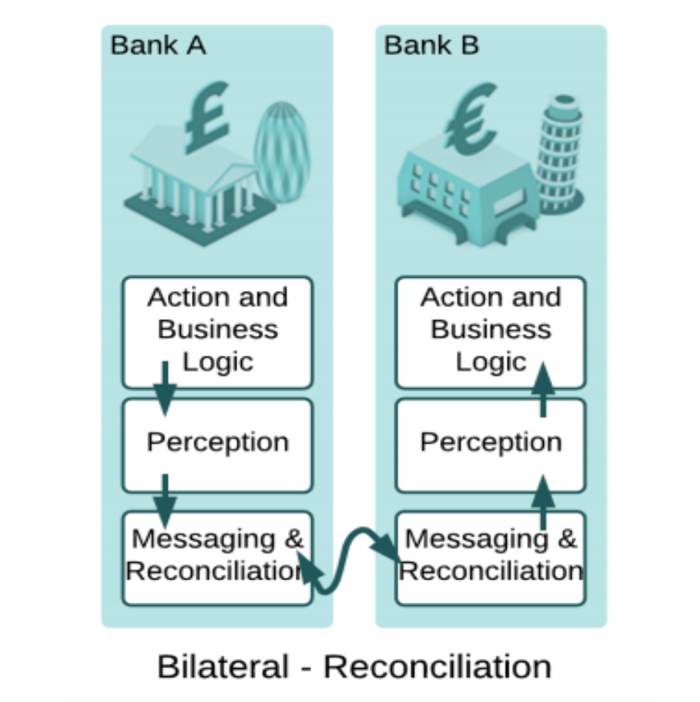
\includegraphics[width=0.7\textwidth]{bilateral-rec.png}
        \caption{Bilateral reconciliation of records, matching transaction details after each party applies its own business logic}
        \label{fig:bilateral}
    \end{subfigure}
    ~
    \begin{subfigure}[b]{0.48\textwidth}
    	\centering
        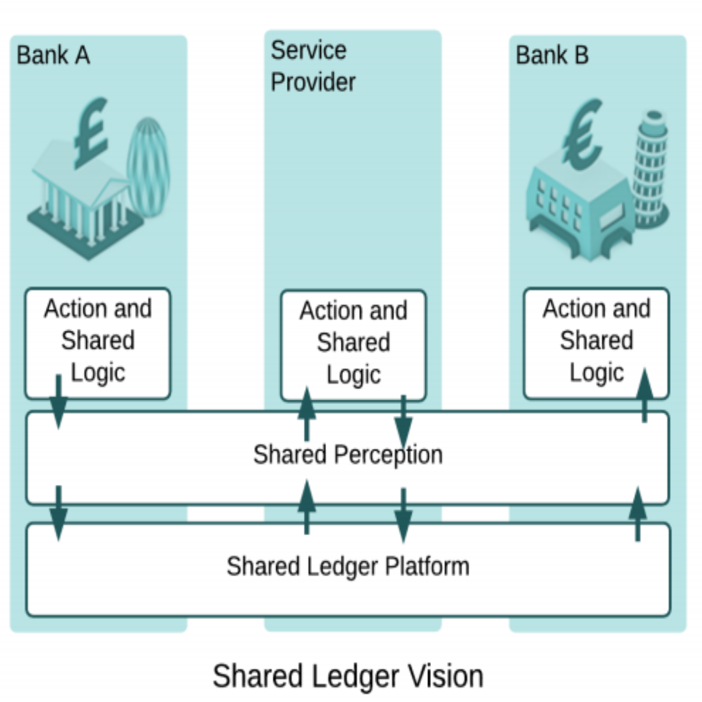
\includegraphics[width=1\textwidth]{shared-ledger.png}
        \caption{Schematic representation of the shared ledger implementation (along with the the technology service provider)}
        \label{fig:shared}
    \end{subfigure}
    \caption{Ledger implementations: traditional vs. ideal solution \cite{Corda:IP}}
    \label{fig:reconciliation}
\end{figure}

In traditional banking systems, it is common for every bank to have its own view of the ledger. This is not the only piece that differs between banks, the business logic implemented having various discrepancies too. To be able to reconciliate records, a messaging system has to be in place. This adds another layer of complexity and potential sources of risk and errors - reconciliations might fail for several reasons (record mismatch, human errors when transferring data over the network). This can be visualised in Figure \ref{fig:bilateral}. However, in the ideal system Alice and Bob are using, this is no longer a problem because of standardisation of protocols and the shared view of the world. A technology service provider would support the common business logic between banks and manage the perception of the data to ensure integrity. This implies that market infrastructure providers would have to come up with competitive ideas instead, shifting the paradigm. This ideology is presented in Figure \ref{fig:shared}.

\subsection{Requirements}
\label{sub:Requirements}
The UK Government Chief Scientific Adviser discusses several characteristics that a blockchain should have for banks to use it \cite{GOVReq}. This paper takes some of these recommendations as high-level requirements, but we will go in more depth to explain what they actually entail (for example, what does `high-performance' actually mean?). 
\\ \\
\textit{High performace and low latency:} There is a proposed speed of at least 100,000 transactions per second \cite{Chinese}. This makes sense in today's context and the rapid developments we are facing. As a comparison, VISA has a peak of 56K TPS \cite{visa}, but only handles on average 2K TPS every day \cite{Scalability}. However, the decision takes into account an increase in trading activity. To be able to assess this in the chosen systems, we also have to take into account latency introduced by other factors (extra nodes in the network, for example) or the bandwidth used. 
\\ \\
\textit{Efficiency and costs:} Institutions have to take into account the cost of implementing the new systems, but also miscellaneous costs such as onboarding. This depends on the learning curve of the introduced system. Therefore, the requirement is to build a system that is intuitive, easy to use. An analysis should be done on the difference between current costs of maintaining antiquated systems and the expected costs for the new system.
\\ \\
\textit{Security and privacy:} The most important characteristic for the financial industry is related to security. There are plenty of ways that information can be leaked and we need to make sure that any vulnerability has been taken care of in a potentially implementable system. Some characteristics that fit this category are: being able to hide transaction information, obfuscating the IPs of the participants, avoiding the identification of participants from the keys the use and retrieving their trading patterns, dispute resolution and the correction of mistakes and the general avoidance of information leakage. 
\\ \\
\textit{Permissioning and memberships:} Related to the previous point, the permissioning system would enhance the privacy of the system. Therefore, we should be talking, at least in the initial form, about a consortium of banks. They would be governed by a superior, objective, trustworthy entity. Any new members would be able to join the consortium after passing important checks related to system requirements and internal security protocols.
\\ \\
\textit{Compliance:} The current banking system has in place several monitoring mechanisms to prevent illegal trading. Among these we can count Know-Your-Customer, Anti-Money Laundering and Anti-Terrorist Funding controls. Some banks are not allowed to trade with certain high-risk countries. All these have to be included in the design of a digital platform that seeks to reinvent the banking world. Moreover, there should be the possibility of having auditors (or audit nodes, as an example) that can monitor every transaction. They can perform checks to ensure the financial reporting is reliable and compliant to applicable laws and regulations \cite{GS:Audit}. The auditing facilities can either be internal (for the company's own monitoring) or external (having a general view of the trading world and the transactions performed). To aid in this process, the system should have timestamping abilities, which are important for determining transaction times, durations and different events. Being a live, real-time system, it is hard to ensure that all clocks are maintained synchronised, so these timestamping facilities should allow for time ranges instead of fixed time points.
\\ \\
\textit{Reliability and persistence:} Clearing Houses are SIPS (Systemically Important Payment Systems). Countries either have a Real-Time Gross Settlement system or there are systems serving multiple countries (the pan-European TARGET2, for example). Their two key elements are the transfer of information between the payer and the payee banks and the settlement, which is considered irrevocable and unconditional \cite{RTGS}. Their criticality means they have to be extremely reliable. As an example, TARGET2 deals with the settlement of around 350.000 transactions daily \cite{TARGET2}, and it is only dealing with the Eurozone. Obviously, this means that replacing such a system will be a big task and the onboarding time will be proportional. A thorough analysis into the reliability of the new system will have to be performed to ensure it is up to the standards banks are looking to achieve.
\\ \\
\textit{Scalability:} The new system will have to be able to incorporate several nodes (the banks). They will represent the consortium that will be able to use the system seamlessly. However, there have to be alternative options for the banks that are not using it. The integration between the two options is of utmost importance to be able to make a smooth transition for the banks who choose to be part of the consortium and to be able to continue normal trading procedures as before. Performance is the characteristic that we have to look at here - will it be affected by the extension of the consortium? A good approach would be to start with a small consortium of banks and gradually extend the network as the system's reputation grows.
\\ \\
\textit{Network types:} The consortium of banks that will operate on the system will have to be linked by a very high-speed network. The way the system will actually be implemented gives more freedom of choice - peer-to-peer, private peer-to-peer or even friend-to-friend (where nodes have direct connections only to other nodes they know). There has to be a guarantee that transactions can happen between nodes situated in different machines or regions. A study into local banks' networks in Italy \cite{Italy:networks} outlines the need for links between banks to further economic performance. Therefore, the network should support connections between nodes that are not directly connected too, to improve productivity. Also, the speed of the connections is important in trading, but does not present a significant importance in the clearing and settlement of trades. 
\\ \\
\textit{Currencies:} Cryptocurrencies have enjoyed public acclaim since the appearance of Bitcoin. However, there are plenty of downsides to them as well. Cryptocurrencies would be traded just like any other currency, meaning that they will have a certain value. This can turn out to be a negative side effect since for some cryptocurrencies their volatility is still too high. Of course, for a system that used blockchain (or a version of it), the usage of cryptocurrencies would be obligatory or recommended. But is this the only option to represent money? Financial constructs could be represented by using a version of fiat money tokens and securities tokens. Fungible assets (mutually interchangeable) can be represented digitally by adopting a certain state the client is in (for example, the state in which he \textit{owns} a certain \textit{fungible asset}). For fiat money, this holds regardless (i.e. a \pounds 5 note will always be worth \pounds 5). As an example, for bitcoin there might not always be the case of fair trade and markets might discriminate based on the bitcoin's ownership history \cite{BC:Fungibility}.
\\ \\
\textit{Reputation systems:} There has to be a voting failure handling for the nodes participating in the system. Do we trust all the nodes? Maybe, but they can still be corrupted (during a possible attack, for example). Therefore, the consensus protocols or mining facilities that evaluate transactions have to be well researched. Moreover, there has to be an analysis into the processing type of these votes - are they done sequentially or in parallel; how many votes are required; what is the granularity level of the voting (per transaction or per ``blocks" of transactions?).
\\ \\
\textit{Wallets:} Every customer should be in possession of a container that has all the assets it owns. This digital container should have the mixed assets of the client. These assets have to be issued previously by a governing authority (a Central Entity, say). 
\\ \\
\textit{Usability:} The new system must be as similar to the previous one in terms of user interface. That being said, banking systems are famous for maintaining the same UI since the beginning of their application, solely for the reason that ``it works". Of course, brokers got used to the looks so, although there will have to be a change to refresh the design and bring it to more modern days, it should be done in such a way to cause as little disruption as possible. The applications developed in this paper will not attempt to fulfill this requirement since there should be a direct collaboration between the potential users and the developers. Hence, the paper only looks at the functionality of the presented systems.
\\ \\
\textit{Reputation and marketing:} Adoption of new techniques and frameworks is controversial in the financial world. Has it been tested enough? Does it feature all the requirements we have? Has it been used before? What are the failure rates and how trustworthy is it? Again, not all of these questions will be answered in this paper, since the system would have to be tested in the real world, at a very large scale, to provide a very high level of certainty. Reputation - the widespread belief that the solution is good and trusted - cannot be easily quantified, so the proposed system will have to have a strong marketing campaign, along with partnering banks which are able to support development. An idea to increase the reputation would be to implement testnets and have experiments done on them by each bank who is thinking about adopting the new system.

\subsection{Distributed Ledgers}
\label{sub:DistributedLedgers}
Many believe that cryptocurrencies (and more importantly, the infrastructure they use) have the potential to ``disrupt" the financial world. They also agree on the fact that the lack of liquidity and their volatility currently represent a major obstacle. However, there is no doubt that the underlying technology of Bitcoin will ``alter the financial landscape" \cite{CMM:RN}. Therefore, we will look at these distributed public ledgers, both the original one and altered versions. The most prevalent type of these is often referred to simply as blockchain.
\\ \\
The most common salient features of blockchains are transparency (everyone can see the transactions on the blockchain) and redundancy (every node has a copy of all the blocks). They often run on P2P networks, use digital currencies and are based on mining to verify the transactions. This presents us with a lot of issues, were we to implement our system on one of the ``common blockchains". We do not desire transparency, we would like individuals' identity to be protected and trades to be private, hidden. Otherwise, the market would easily be influenced from a simple analysis of trades that took place. Moreover, the redundancy in every node does not suit us - it is a problem of cost and scalability, although methods have been designed to prevent any issues that could arise. Mining as a method of verification is costly as well, since it is based on the Proof of Work (discussed below) and \textit{rewards} the nodes who contribute computation power. In a financial blockchain scenario, we would not have to worry about monetary compensation, since all the nodes are \textit{fairly} working towards the same goal. The peer-to-peer network might not be suitable for our purposes since its design principle of avoiding all regulations is in direct contradiction with one of the requirements described. The use of cryptocurrencies serves the purpose of keeping the integrity of the original blockchain's principle. However, they can easily be replaced by digital references to cash liquidity or other assets.
\\ \\
This showcases the need for creating a purpose-built blockchain-based solution, instead of adapting existing general ones. We will look in more depth into Bitcoin's original blockchain in a subsequent section. 
\\ \\
To offer some insight into the verification techniques present at the moment, we will now look at the two popular ways to perform validity checks: mining (via Proof of Work) and Proof of Stake. To be noted is that not all the presented systems feature such a validity check. For example, Corda employs notary nodes which are discussed in the section dedicated to this system, along with their benefits.

\subsubsection{Proof of Work versus Proof of Stake}
\label{sub:powpos}
\textbf{Proof of Work} uses the power of computation to verify transactions. What this means is that nodes ``vote" the correct version of transaction history by contributing their resources in calculating very rare hashes \cite{PWPS}. Such a system needs to have 51\% of the total power to be validated, protecting against malicious users in this way. One would be able to attack the system by gathering more than half of the network hash rate - and the assumption is that this can never happen. Since there is a reward for the contribution, this ``mining", it is considered to be more profitable to use the computation power to verify transactions that to try to attack the system. However, there are some points that we should consider here. First of all, there is currently an upper bound on the number of bitcoins to be created and currently 76.9\% of all bitcoins have already been mined \cite{BC:UB}. This means that once the cap is reached, miners will no longer be rewarded in new bitcoins, but in transaction fees (possibly much less profitable). Another issue to look at in the case of Proof of Work is that nodes are ``devouring energy in the race for mining profit" \cite{PoW}. There should be an alternative that limits this energy consumption and is, in general, more eco-friendly. The algorithm is not final, providing only a probabilistic approximation which does not fit the standards of the financial system \cite{Corda:TP}.
\\ \\
An alternative solution is considered \textbf{Proof of Stake} \cite{PWPS}. The concept is that instead of basing the votes on the limited \textit{computational} resources, they can be based on the limited \textit{coins}. Therefore, the ticket you are ``paying" to be able to vote is composed of the coins you own. Again, the same concepts apply - to be able to sign a transaction, you need 51\% of the existing coins. The benefits of this type of proof are related to saving energy (no computation power required) and attacks become more expensive, since we would have to buy 51\% of the coins (and the market would react by price appreciation, making the purchase expensive and effectively pointless). The limit is no longer defined by the total computational power, but by the total number of coins people have in their wallets. Unfortunately, this is not without fault. One possible attack is related to double-spending, because Proof of Stake allows to mine different versions of the blockchain \textit{simultaneously}. Also, since the private keys for money already spent are ``useless", there might be people tempted to accept money for them. An attacker can rewrite the history of the blockchain by mining with the old keys though at a certain point in the past. He is the one receiving all the rewards since he would technically own 100\% of the coins in his version of the blockchain. At some point, this alternative version of the blockchain will catch up to the real version and have a larger number of blocks. But there is nothing preventing the network from switching to the malicious, manufactured blockchain, since technically it is the more recent one, with more transactions recorded. From this point onwards, the malicious user owns more most of the coins in the network and can perform any attacks.
\\ \\
There have been developments in the implementation of both types of proof and their security has been improved (PeerCoin performs regular checkpoints preventing branching in Proof of Stake \cite{PWPS}). There have also appeared some hybrid combinations of the two such as Proof of Activity or Proof of Burn \cite{PAPB}. However, these are still theoretical approaches, so they cannot be used in industry systems.
\subsection{Available systems} 
\label{sub:AvailableSystems}
There are several industrial-grade projects that have taken off since the appearance of the first implementation of a distributed ledger. Some of them are general-purpose solutions, while others look specifically at blockchains for the financial industry. However, it is not the case that the distributed ledger has to be a blockchain. This section aims to look at how the requirements established above are satisfied in each of the systems researched. 

\subsubsection{Some insufficient solutions}
\label{sub:Insufficient}
\textit{Bitcoin's blockchain:} The most popular blockchain and cryptocurrency (its market cap being more than 17 times larger than the next most used cryptocurrency \cite{BC:MC}). But is it an appropriate base for applications able to revolutionise the financial world? Arguably, no. One of the biggest problems we would be facing by using this implementation is the performance. Currently, the peak number of transactions per second is 7 (not comparable to the 100K TPS we require for a system to be feasible for the financial industry). It is clear that unless drastical improvements are being executed, this BC does not fit our purpose. Even so, there are more hurdles that have to be overcome in order for this to become a possible solution. However, looking at the original implementation, it is a lot easier for us to compare the subsequent solutions. 
\\ \\
The ledger offered by Bitcoin's blockchain is public. Everyone has access to the history of transactions and although they are cryptographically protected, there are possible identity leaks. For example, there can be an attack aimed at tracking spending habits for certain clients. The clients are identified by their keys, but nothing more is actually needed in this case - these patterns could influence the markets \textit{or} give an insight into what other people are trading, when and how. There are no permissioning systems in place, so anyone could participate in adding blocks to the blockchain (unless a membership subsystem is formed). Moreover, since this BC functions by employing Proof of Work as the verification method, there would have to be a consortium of dedicated miners able to support its activity. That means that there will be extra costs from providing computational power, as well as worries about the source of computational power (for example, would it be possible to use a botnet to mine?).
\\ \\
\textit{Hydrachain and BeihangChain:} Hydrachain is a private BC based on Ethereum and developed with the purpose of serving financial scenarios \cite{Chinese}. From the point of view of performance, it is an upgrade on Bitcoin's BC, but having 1K TPS is still not up to the standards desired. It has most of the same features of general blockchains, with some particularly interesting characteristics to note. Blocks are only created by ``leaders" (which would have to be defined as a superior entity in our financial system - potentially a Central Bank). Voting is done on each new block, by using Byzantine voting and if a block receives 1/3 of the votes, there will be a new vote cast. 
\\ \\
Another private chain is BeihangChain, that performs concurrent voting and data collection \cite{Chinese}. This speeds up the process and reaches (at best) 24K TPS. Any node is able to create new blocks, but the voting in this BC is more sophisticated. Not only are new blocks being voted on, but also each transaction, increasing the number of messages being transferred between nodes.
\\ \\
These approaches are getting closer to our goal, but they have been developed to take care of individual scenarios at a time - a BC for trading and a BC for account information. However, we are not seeking to build blockchains that completely support the banking system. Yes, this could be possible in the future, but replacing every system should be a gradual approach. To use one of these 2 BCs for Clearing and Settlement is possible, but there are 2 main issues: the tests performed have been developed on controlled environments and the source code is not available to the public (making it hard to extend and test it). Therefore, we will not be considering these mostly theoretical approaches further.
\\ \\
\textit{BigchainDB:} This approach claims to ``fill a gap in the decentralisation ecosystem" \cite{DBC}. It boasts amazing performance (1 million writes per second throughput) and low latency. Indeed, this is a scalable option and does fit most of our requirements: private, permissioned and performant! However, many have criticised its design for being fundamentally flawed. This is because all nodes are using the same RethinkDB cluster (a distributed database) which leads to extreme fragility. If, for example, one node becomes corrupted, it can simply \textit{dropTable} on the cluster, leading the whole system to crash \cite{Sewer}. Obviously, we are not expecting any of the nodes in the consortium to be hijacked, since they are permissioned after a long series of checks. However, security is not perfect and there will always be vulnerabilities and potential zero-days. The financial world cannot take this risk, therefore, from a security perspective, this solution is infeasible.
\begin{comment}
\begin{table}[]
\centering
\caption{My caption}
\label{my-label}
\resizebox{\textwidth}{!}{%
\begin{tabular}{@{}cccc@{}}
\toprule
\rowcolor[HTML]{C0C0C0} 
{\color[HTML]{333333} \textbf{Requirements}} & {\color[HTML]{333333} \textbf{Bitcoin}} & {\color[HTML]{333333} \textbf{\begin{tabular}[c]{@{}c@{}}Hydrachain and\\ BeihangChain\end{tabular}}} & {\color[HTML]{333333} \textbf{BigchainDB}} \\ \midrule
\textbf{Performance} & low (7 TPS) & medium (1K TPS) & high \\
\textbf{\begin{tabular}[c]{@{}c@{}}Security, privacy\\ and permissioning\end{tabular}} & \begin{tabular}[c]{@{}c@{}}transactions are\\ public, seen by all\end{tabular} & \begin{tabular}[c]{@{}c@{}}developed for \\ financial purposes\end{tabular} & some permissioning \\
\textbf{Compliance} & \begin{tabular}[c]{@{}c@{}}no protocols\\ implemented\end{tabular} & \begin{tabular}[c]{@{}c@{}}basic protocols \\ implemented\end{tabular} & \begin{tabular}[c]{@{}c@{}}no protocols\\ implemented\end{tabular} \\
\textbf{Reliability} & high & unknown & issues reported \\
\textbf{Costs} & \begin{tabular}[c]{@{}c@{}}mining and\\ transaction fees\end{tabular} & low & low \\ \bottomrule
\end{tabular}%
}
\end{table}
\label{tab:comp1}
\end{comment}
\subsubsection{BitShares and Stellar}
\label{sub:BSS}
\textit{BitShares} is a platform for financial smart contracts, developed specifically to address problems in traditional cryptocurrencies such as high volatility \cite{BS:TP}. The founders intended to provide tools for the creation of both market pegged assets and user-issued assets. Their practical payment solution does not rely on creating a price-stable asset, which historically proved to be dangerous because of issuers that become bankrupt. Instead, it uses their proprietary cryptocurrency as collateral in contracts. The cryptocurrency, \textit{SmartCoins} has a value pegged to another asset (US dollars or gold, for example). 
\\ \\
The system has plenty of advantages, offering ``financial instruments for anyone to use with low barriers to entry". As a system of verification, it uses a Delegated Proof of Stake, which is the most efficient consensus protocol available \cite{BS:DPOS}. Because of it, the performance is also different than the systems presented above - it is able to perform 100K TPS if the infrastructure is being accounted for (i.e. the system is able to reach the highest level only if the network connections and node structures are of a high standard) \cite{BS:tech}. It also incorporates compliance techniques such as KYC, which were presented in the requirement list. To appeal to the corporate world, it does enable dynamic account permissions which eliminates some of the risk of hacking compared to the public ledger. 
\\ \\
However, there are some downsides to this as well. Because the system introduces a new cryptocurrency, there is again concern for price manipulation and market influencing. This is taken care of by pricing the risk into the premium paid, but there have not been tests on whether this is able to cause serious trouble in a real trading environment. Moreover, every transaction will incur a fee. This makes sense from the point of view of the company, because it has to be self-sustaining. But in the financial context, the goal should be to have a system that is able to encompass all the current business features without additional costs (other than the ones for running the machines/servers). This would disadvantage companies with large trading volumes. Even though the fees for BitShares would be priced into the fees of the brokers for handling transactions, a further cost-benefit analysis would have to be carried out and compared with other solutions.
\\ \\
\textit{Stellar} is a similar concept to BitShares, with a similar performance in terms of transactions. It uses a different consensus protocol, the Stellar Consensus Protocol (also named the Federated Byzantine Agreement model) which adds flexible trust to the classic Proof of Stake \cite{Stellar:TP}. It operates with an inflationary currency (Lumens) which facilitates multi-currency transactions and hinders DDoS attacks (because every transaction has a fee). However, this BC is focused on managing micropayments and is specifically targeting individuals, encouraging an expansion of the banking systems to the underbanked \cite{Stellar:docs}. Although it would be possible to focus on the conversion of Stellar into a corporate-facing company, there are currently other alternatives that seemed more appealing.

\subsubsection{Ripple}
\label{sub:Ripple}
Ripple is the second largest blockchain in terms of market capitalisation, after Bitcoin. Its distributed financial technology allows institutions to reduce delays when performing transactions and ensure their clearing \cite{Ripple:TP}. Through this on-demand payment, clearing risk is reduced and efficiency is improved. Moreover, the compliance processes related to tracking and investigation are aided by the infrastructure (the financial institution remains responsible for the onboarding process of clients). The diagram shows the structure of the Ripple system. To incorporate it in banks' systems, they have to be linked to a Ripple Connect node. The messaging (consisting of payment instructions, exchange fees, customer information and payment confirmations) is done directly between these nodes. For the settlement of the transactions, the nodes employ the Ripple Network (validators that perform cryptographical checks on the validity of the data) which also confirms the transaction to all parties involved.
\begin{figure}[H]
\centering
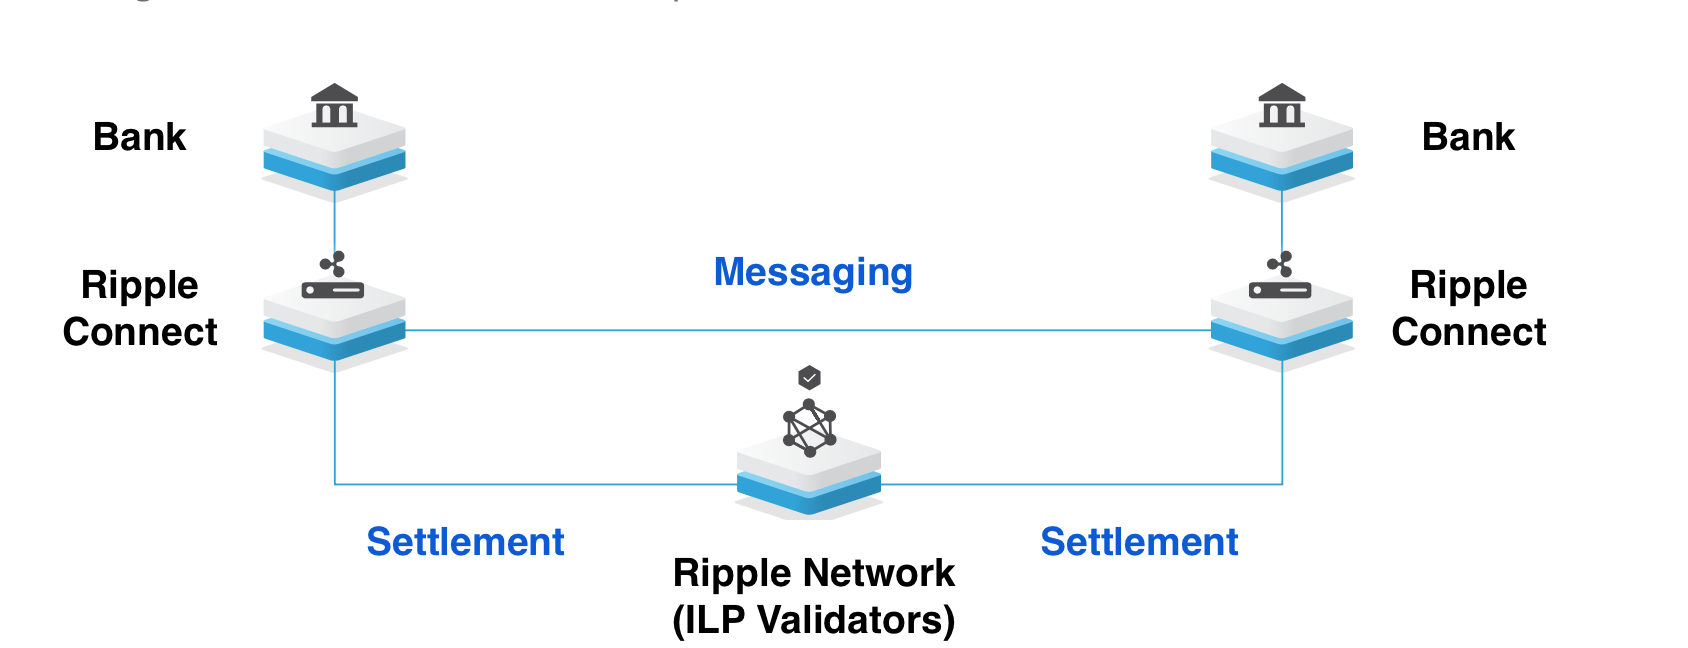
\includegraphics[width=1\textwidth]{ripple.png}
\caption{Ripple node overview \cite{Ripple:TP}}
\centering
\label{fig:Ripple}
\end{figure}

Ripple becomes a technology service provider in this case and banks are meant to have the Ripple Connect incorporated to be able to settle transactions over the network. The infrastructure is highly configurable and makes use of the Interledger Payment (ILP) validators (a byzantine-fault tolerant consensus algorithm) \cite{Ripple:ILP} \cite{Ripple:CP}. This protocol does not have access to the payment details, it cryptographically verifies whether the conditions for validity are met. 
\\ \\
The setup of the Ripple system is done by having a separate Ripple ILP Ledger which acts as a suspense account tracking the state of the funds. The process flow involves several API requests to Ripple Connect (getting the quotes, accepting them and locking them, for example). The actual payment process consists of 3 stages: sending the payment from the originating bank, executing the transfer over the Interledger Protocol and settling it, and receiving the payment at the beneficiary bank \cite{Ripple:TP}.
\\ \\
However, as it happens in Stellar, Ripple also uses its own cryptocurrency to stave off attacks by demanding a fractional amount for every payment. There are other concerns or criticisms against Ripple as well. In a review done by Jo Lang \cite{JoLang} there were issues raised such as the possibility of a fork in case more than 20\% of the network nodes do not agree on the validation of a transaction. All that being said, considering the system has been already in place for a few years, it has been subjected to higher amounts of peer reviews and reports contributing to the overall enhancement of the Ripple solution.
%TODO:Provide a summary of why none of them work.
\subsubsection{Corda}
\label{sub:Corda}
The final system to be presented in this section is Corda - born from the desire to have a blockchain-based solution that specifically caters to the financial industry and that is developed in concordance with expert guidance from the domain. In this section, I will discuss a high-level introduction into the Corda ecosystem, present which requirements it is able to fulfill, determine the challenges in using this system and explore potential ways to expand on the existing codebase.
\\ \\
The blockchain paradigm has the potential to revolutionise many areas - health services, elections and transparency in supply chains. However, the public nature of the ledger is frowned upon (at least for now) in the financial world. Corda's proposition is based off the blockchain ideas, but the execution tries to maintain global databases at the core of the processes. Therefore, it puts forward the idea of a ``distributed ledger made up of mutually distrusting nodes" which enables the recording of different transactions in a single global database \cite{Corda:IP}. The platform is also abiding by the financial institutions desires of having a regulated environment. Moreover, by using the shared ledger and having the same perceptions about the data existent (transaction details, records, etc), there is no risk in mismatching records and therefore, no need for reconciliation. DIAGRAM
\\ \\
Instead of directly replacing all the systems with Corda, the founders seek a phased approach. Therefore, not only does the platform allow gradual integration, but it supports the addition of new nodes or combining networks based on applicability potential. This links well with the usability criterion, through which we want to ensure that both the engineers who have the job to integrate this system into the current banking processes and the users are going to be happy about the changes.
\\ \\
From a high-level perspective, the end-goal is to have allow parties to record and manage agreements reliably, privately and authoritatively \cite{Corda:IP}. The global ledger will have a distributed physical appearance, but will act as one logical component. The records contained on the ledger should be legally binding and open for investigation from compliance and regulatory entities. From the point of view of privacy, access to data is intended to be granted only to those who need it (therefore, the system works on a need-to-know basis) - the parties who take part in a transaction and the regulator entities present in the system. Therefore, instead of broadcasting transactions like in the typical blockchain systems, Corda makes use of the concept of \textit{flows} - multi-step transaction building protocols. These manage the transaction structure and ensure that all the requirements for a smart contract are met. For example, we would use a flow to perform a transaction between Bank A and Bank B and add a flow that ensures there is a regulatory entity participant in the process too.
\\ \\
At the requirement fulfillment level, we can look at the most important aspects that Corda satisfies. Being specialised for use within regulated banking institutions and developed under the assumption of an adversarial security environment, protection of data and privacy have been critical in Corda's implementation. Data is shared on a need-to-know basis, therefore not everyone has access to all the records. This increases security because Bank C should not have access to a trade that took place between Bank A and Bank B. Regulatory nodes have the option to see what the transaction details are by adding special commands to the transactions (and the assumption is that any transaction will be overseen by at least one regulatory node). Corda does not employ a mining mechanism for the verification of data, nor a Proof-of-Stake approach. Instead, it uses the concept of ``pluggable services". The default for now is the RAFT algorithm which is formally proven safe \cite{raft}, but this can be replaced by Byzantine fault tolerance systems. Moreover, the details of the transactions are kept private - using Merkle trees, they can be ``torn off" and only the root of the transaction will be validated cryptographically (the rest of the information is useless for the signing authorities) \cite{Corda:TP}. 
\\ \\
Performance-wise, data is no longer completely replicated in each node, but there is a single reliable source available. This adds another layer of efficiency and reduces delays introduced by the necessity of data duplication. Corda works with smart contracts which define the business logic of the ledger and enforce the validity of transactions. The JVM used in Corda is extended with a custom sandbox that restricts usage by enforcing security requirements and deterministic execution \cite{Corda:IP}. However, there have not been any tests regarding the number of transactions per second or the load a node can resist until now. These are planned to be performed as part of this project, providing both quantitative and qualitative results to support any claims made.
\\ \\
The ideal scenario would see a consortium of banks running Corda, after specific permissioning requests from each institution have been analysed and granted. The permissioning service would sign off the requests and add the new party to the semi-private network. One important requirement would be for all of them to contribute to the network in an equal manner (i.e. they provide nodes that run on servers that match the hardware requirements). This way, the standards of the consortium will be kept high for everyone to benefit from the Corda integration. There will have to be a cost analysis that takes into account the integration of the new system, onboarding the brokers on it and maintenance needs. 
\\ \\
To be able to replace the Clearing Houses, Corda needs to prove it's reliable and persistent when dealing with transactions and contracts. Nodes are backed by a relational database which can be joined with data from the ledger, on request. Wallets (called \textit{vaults} in Corda) have the different assets that customers own and can also be accessed with SQL queries.  There will be further analysis into how the reliability is provided with Corda, as well as looking into data storage, in future sections. 
\\ \\
From the business logic perspective, transactions follow the Bitcoin structure, having inputs, outputs and signatures. The ledger records the ownership of assets through states. Corda does not use a cryptocurrency to represent other assets, especially cash. Therefore, the issue that may arise in this case is related to national fiat currencies which might not be fungible in some cases (because unless the issuer is a Central Bank, it might go bankrupt) \cite{Corda:TP}. This will be studied further in the developed applications, looking at obligations, trades, interest swaps and contract constraints that would make use of all of Corda's features. We will also be looking at asset representation and integration with cryptoasset tokens or cryptocurrencies.
\\ \\
As seen above, there are a lot of unknowns in Corda. This is because its development was started in 2016, the source code becoming open-sourced in November 2016 to enable contributions from anyone willing to help. Although many of its premises are not implemented yet, the system in its current state is promising enough to constitute the basis for this project. It has to be noted that any tests performed on Corda code will not take into account possible optimisations that are expected to be done to the system after the implementation of all stated goals. The biggest challenge related to this project is the volatility of the codebase - development is in progress, therefore changes might occur at any point during the project. Along with these, there could be released similar applications or tests as the ones this project is attempting to present. Therefore, an active research will still take place even after the initial phase in which information about the system was gathered and any modifications and updates will be clearly signposted throughout the next sections. 
\\ \\
The potential ways to build on this system and present a prototype align well with the goals of the paper. First of all, a suite of applications targeted at particular concepts present in Corda will be developed. These will test modularly the properties of Corda and how or if they satisfy the requirements. Besides the distributed ledger system, Corda also provides developers the option of building their own CorDapps, which are basically templates for different pieces of functionality one might require in a financial context. Therefore, the applications that will be created during this project might take the form of a CorDapp, if needed. These applications are mainly aimed at analysis the following:
\begin{enumerate}
\item \textit{Performance metrics}: transactions per second and load testing
\item \textit{Feature corectness and implementation stability}: aims to demonstrate persistence via the database, security, latency issues arising from scaling up the system or from the usage of different features, and asset class representations
\item \textit{Compliance}: latency introduced by regulatory entities, network packet routing 
\end{enumerate}
There will be a theoretical analysis looking at performance metrics, as well as statistical security proofs to ensure the corectness of consensus protocols. Finally, there will be an educational demonstrative application that will encompass all the major features Corda has to offer. This should take the form of a CorDapp, with a user interface based on the ones already used throughout the project. Since these are different for each demo application already available, the final product should merge all the current features and enrich the application with new concepts described in subsequent sections. Therefore, to support this, this project will also involve writing contracts containing various business logic constructs, commercial papers and legal attachments.
\\ \\
An important thing to note is that in the case of succeeding to satisfy all the remaining technical requirements, there can be no study into the reputation and marketability of Corda.
\newpage
\section{Design and Implementation}
\label{sec:DesignImplementation}
\subsection{Network pre-analysis}
\label{sub:Network}
The most important feature in a distributed ledger is the possibility of spreading out the nodes on different machines, in different subnets, in different regions. The demo applications developed on Corda have been built so they can run on only one machine. Therefore, the first step was to distribute the nodes. However, this functionality is currently not automated. The node configurations can be accessed and modified, but this process is manual for the time being. Nevertheless, I have attempted the distribution of nodes on several machines by modifing the configurations. What I have found out at this point is that connections can be indeed established if the machines are on the same subnet. This behaviour can be seen in the following figure, with the 3 nodes being run on 2 Azure machines (Controller, Bank B and Bank C are on machine1 and Bank A is on machine2, having different IPs on the same subnet). Bank A and the notary service can be seen running on 2 different machines (and they have different IPs). 
\begin{figure}[H]
\centering
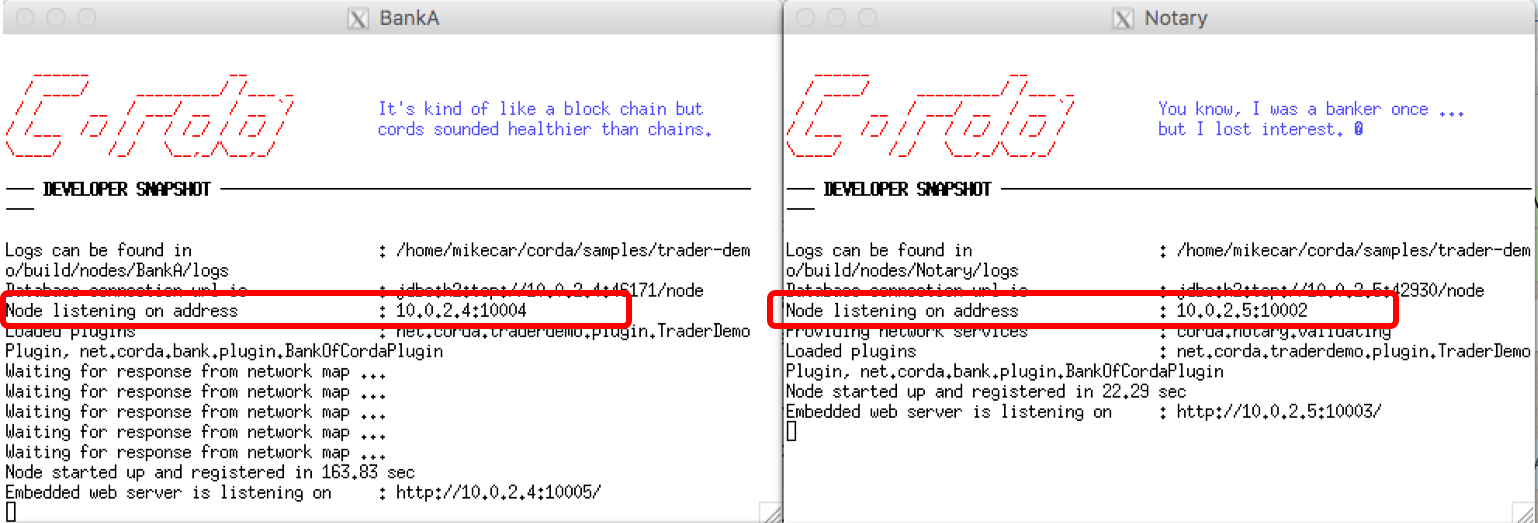
\includegraphics[width=1\textwidth]{diffips.png}
\caption{Distribution of nodes on 2 machines (different IPs)}
\centering
\label{fig:IPs}
\end{figure}

However, no trade is able to take place between the 2 machines at this moment. By trade, here, I am referring to the ``Trader demo" application presented in the Corda docs \cite{Corda:docs}. A similar approach was attempted using the CorDapp-template \cite{Corda:template}. Connections function as well when machines are on the same subnet. IOUs can now also be logged via HTTP requests and there are several web points served for the nodes. An example of an IOU submitted via the HTTP API can be seen in figure \ref{fig:CNT}, along with its results in figure \ref{fig:NT}. 
\begin{figure}[H]
\centering
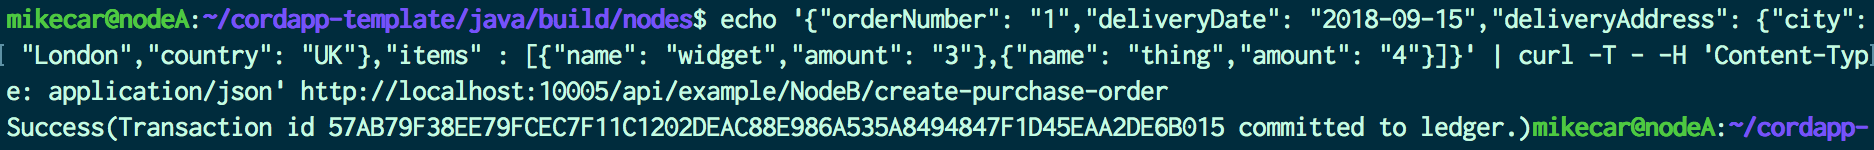
\includegraphics[width=1\textwidth]{httpreq.png}
\caption{HTTP example request}
\centering
\label{fig:CNT}
\end{figure}
The nodes first register with the notary service. After the HTTP request is made, node A constructs the proposed order (and the process can be seen in the green box). After that, the response from node B is given (blue box) and the transaction is recorded in the vault.
\begin{figure}[H]
\centering
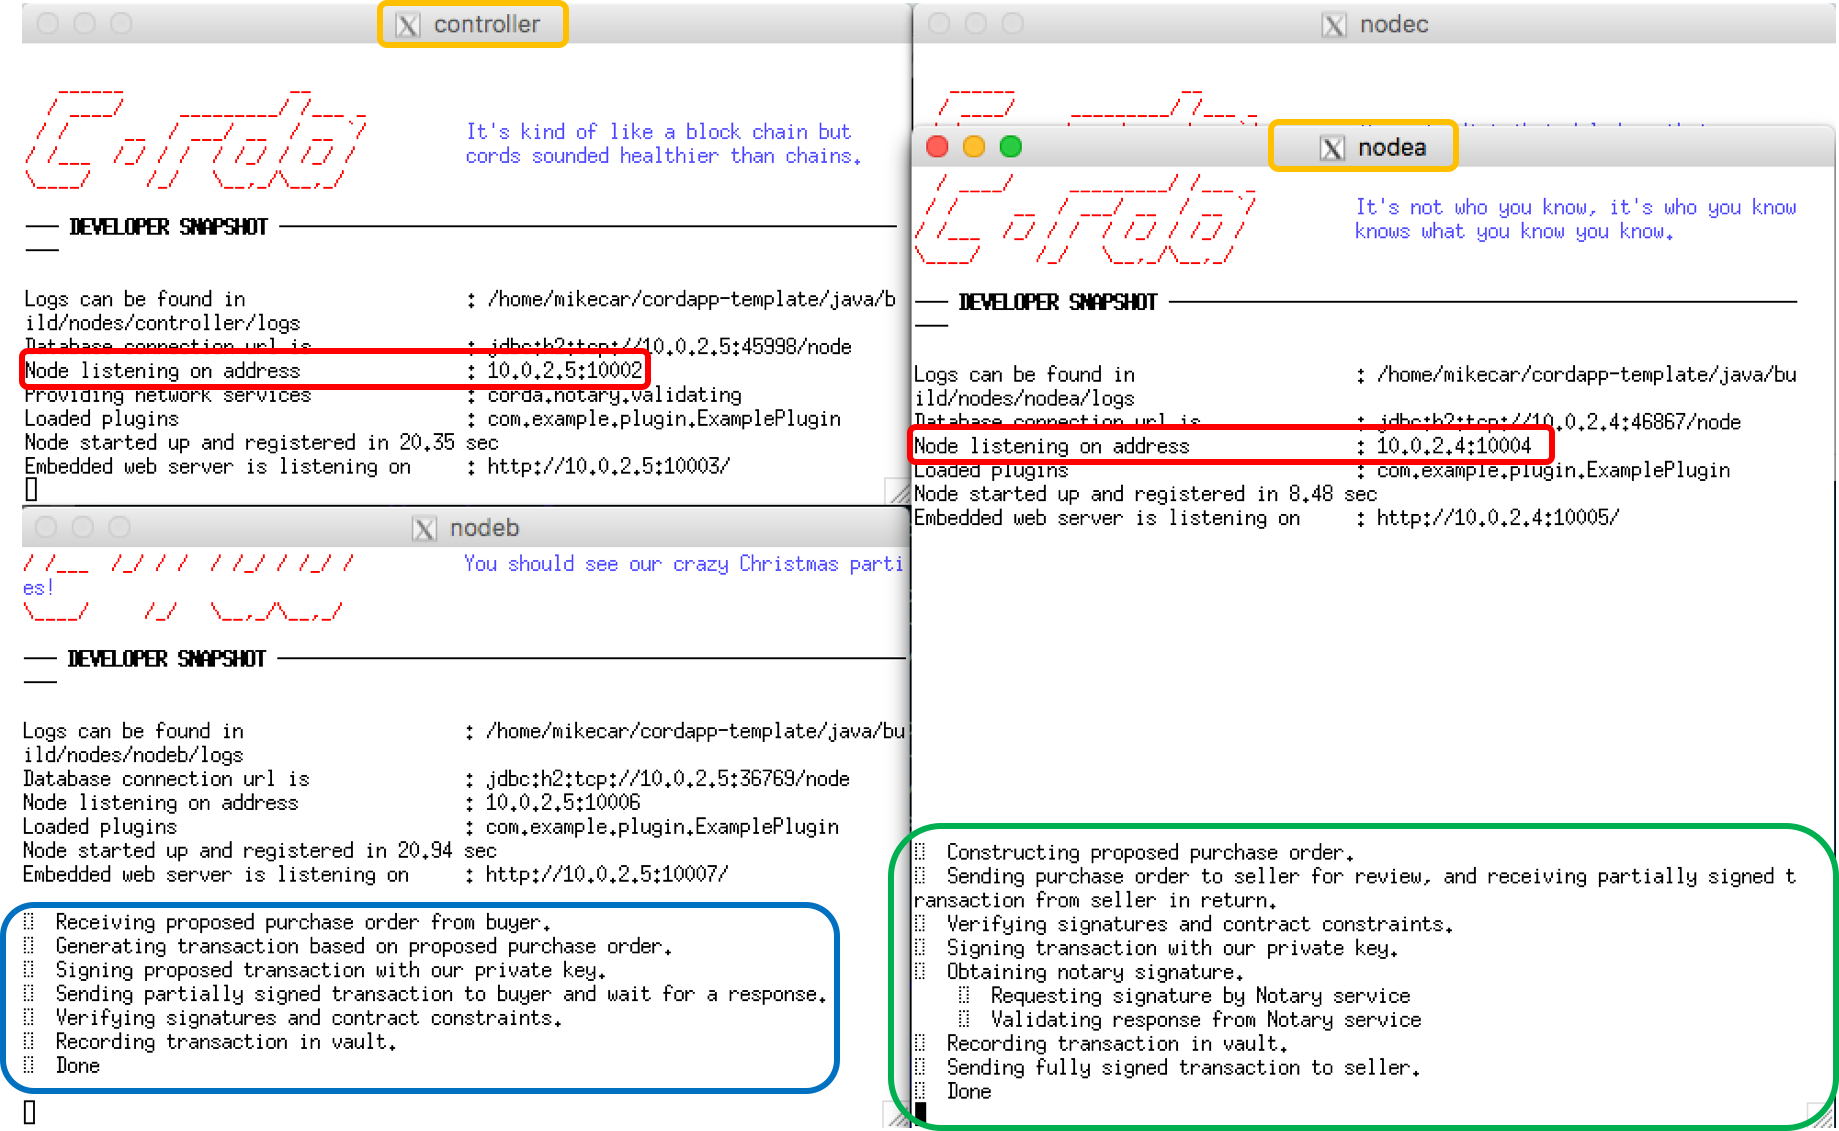
\includegraphics[width=1\textwidth]{cordanodes.png}
\caption{Corda network test}
\centering
\label{fig:NT}
\end{figure}

Finally, an attempt to move nodes on machines that are not on the same subnet has been made. However, after contacting the developers I discovered this behaviour is not yet completely defined. Therefore, this point will be the subject for more research on how to make nodes communicate correctly over the network, even when they are not in the same subnet.
\subsection{Load testing}
\label{sub:LoadTesting}
Load testing can be performed on nodes by applying random stress tests which disrupt different resources. This enables us to study the behaviour of nodes in highly stressful conditions and learn how these can influence their usage. There are several configurations already in place, but no practical test has been yet performed. This will tie in with the performance applications developed.
\newpage
\section{Timeline}
The first month after the assignment of the project was focused on gathering research pieces about the topic. Being a very vague title, I had complete freedom in the opportunity to branch out and explore the sides of Blockchain that interested me the most. Therefore, I chose the area of trade clearing because of my particular interest for the financial world. More research followed, looking at the current state of the art, the salient features of each system and choosing the best one to work with. It was clear that to achieve a good piece of work, I would have to base my work on an existing infrastructure. After studying in-depth BitShares, Ripple and Corda, I decided that BitShares does not serve well my purpose (having an obligatory cryptocurrency attached).
\\ \\
The difference between Ripple and Corda was that the latter gave more freedom to build my own way around the current infrastructure. Being open source, it is much easier to go through the code and modify it as I see fit, rather than having to use an inflexible API. Therefore, although it came with plenty of challenges (a lot of features are not implemented or tested yet), Corda was the best choice. 
\\ \\
The next step was to decide exactly which part of the trading cycle I want to focus on: execution, clearing, settlement, reconciliation? The decision did not come easily, because the entire system needs to be somehow updated to be able to satify the new requirements. Therefore, the paper will present how each step in the trading cycle will be modified to include the adoption of such a system. The plan was to find out what I want to do, what there is available and what can be implemented by the end of January. The decision was to create some small applications showcasing Corda's features and testing different characteristics. One of the apps will be testing the load of the nodes. Another one will demonstrate persistence via the h2 database, compliance, security and the representation of asset classes in a wallet. An application will deal with testing latencies introduced by other nodes, notaries or oracles. Finally, there will be an app testing the distribution of nodes and the routing of packets over the network.
\\ \\
The are plenty of features that cannot be tested directly. For those, a theoretical approach will be taken. Among the characteristics which will be evaluated theoretically are: the number of transactions per second, the repudiation problems and how nodes deal with voting failure and networking (in conjunction with the last application mentioned).
\\ \\
To put everything into context and prove the system is usable, the demo CorDapp will use the interface provided by Corda already and enrich it withb other required features. This means that there will be a suite of contacts and commercial papers written to satisfy the needs of a customer (although in a basic format, at least initially). 
\\ \\
Until the end of March, the small applications should be in place or in an advanced stage (provided all the required infrastructure needed for them exists, otherwise that might delay this part). For the subsequent months, the main focus should be on the theoretical parts of the system (keeping in mind it has not been yet optimised for performance). Also, the bulk of the work will be done for the CorDapp which will be the extensive practical component of the paper. Investigations should be done throughout into what is not implemented and whether it can be bypassed or not. By the end of May, the project should be very well defined and its scope should capture all the requirements presented in the background section, either practically or theoretically. 
\\ \\
For the last month, June, most of the time should be dedicated to writing the report and performing any leftover statistical analysis that would enrich the proofs given. Of course, there should also be time for any final touches and the final presentation that follows. 
\\ \\
There are plenty of challenges the project might face, especially since Corda is in an ongoing development process. However, any piece of work done for this paper that could contribute to the system will be presented. 
\\ \\
Although the plans for the project are somewhat hopeful, if time allows there are several extensions that can be made. Considering Corda's contracts can be written in either Java or Kotlin, a good idea would be to demonstrate this duality by writing some of the CorDapp contracts in both languages. This follows in the Corda developers' footprints and it would make it easier for other developers to become familiar with Corda and the contracts that can be written in it. Another idea would be to perform a more in-depth comparison between Corda and the next best system (possibly Ripple or Stellar). However, this would require more time than currently available, but would act as a great extension on this current paper.
\newpage
\section{Evaluation}
The evaluation of the project follows very much the project plan. The research done for the project has been extensive enough to gather in-depth knowledge about the subject. But it is still important to demonstrate that the requirements presented in the background section have been achieved. And, for those that haven't, show the reasoning behind why it went wrong or why it could not have been done. To succeed in the project, the small applications presented in the Project Plan would have to be functional, confirming or refuting the claims made beforehand. The theoretical analysis should be extensive enough to cover all important aspects presented that cannot be practically tested. Finally, the CorDapp should be a functional piece of software that can be used by people without having explicit knowledge about Corda, its infrastructure or what every component is doing. The evaluation will be supported throughout by statistical proofs.
\\ \\
There are qualitative aspects that are hard to measure, such as ease of use. For this, the final CorDapp should be completed with time to spare, to be able to be circulated among peers (both from the Computing department and outside of it) for direct user testing. Another good way to test its usability would be circulating it among people who actually use such systems in their daily job, but it should be noted that the planned CorDapp will not try to mimic all aspects related to trading. Although useful, their feedback would not be complete unless the final demo application manages to include the entire suite of financial instruments and operations that can be performed. 
\\ \\
There is also the case in which the analysis may uncover the fact that a requirement is infeasible in the Corda-based system. To successfuly navigate this problem, I would have to either find an alternative that can still satisfy the requirement or pivot the project in such a way that the application of the Corda-based system to the financial world would have a smaller impact than the initial planned one. However, this should not happen because the team of developers at the root of Corda work very closely with people from the industry. Again, any such discovery will be prompted to the team for discussion and the possibility of resolution.
\newpage
\section{Bibliography}
\bibliography{mybib}
\bibliographystyle{unsrt}

\end{document}
%%% Local Variables: 
%%% mode: latex
%%% TeX-master: t
%%% End: 
